\documentclass{article}

\usepackage{graphicx}
\usepackage{multirow}

\title{Note: Neural Networks}
\author{Sun Zhao}

\begin{document}
\maketitle
\newpage

\section{Representation}
Brain makes human to learn and gain knowledge. So, what's the structure inside brain and how does brain learn? The answer is neural networks. In biology, neural networks inside our brains consist of billions of neurons, each of which can produce and transfer biological information to others and receive from others too. In machine learning field, neural networks are algorithms that mimic our brain's neural networks. Fig. \ref{neuron_model} shows a simplest neuron having several inputs and one output. There are weights/parmeters on each edge between neurons to represent how strong the connection is. Each neuron collects all the weighted inputs, performs self-defined calculation and produces weighted output. We use an activation function to define the calculation performed on each neuron. Fig .\ref{logistic_neuron_unit} shows a logistic neuron consisting of a sigmoid activation function and an extra bias unit of $x_{0}$. Fig. \ref{neural_networks} shows a typical neural networks including input layer, hidden layer and output layer. Neurons between layer i and layer i +1 are pair-wise connected. Calculations performed on each neuron are shown in the bottom of Fig. \ref{neural_networks}.
\begin{figure}[ht]
  \centering
  % Requires \usepackage{graphicx}
  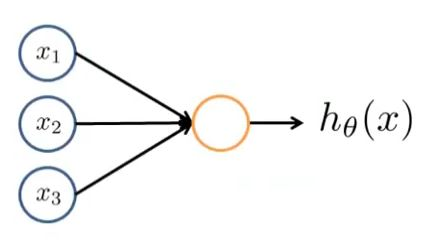
\includegraphics[width=3cm]{Figure1.jpg}\\
  \caption{Neuron Model}\label{neuron_model}
\end{figure}
\begin{figure}[ht]
  \centering
  % Requires \usepackage{graphicx}
  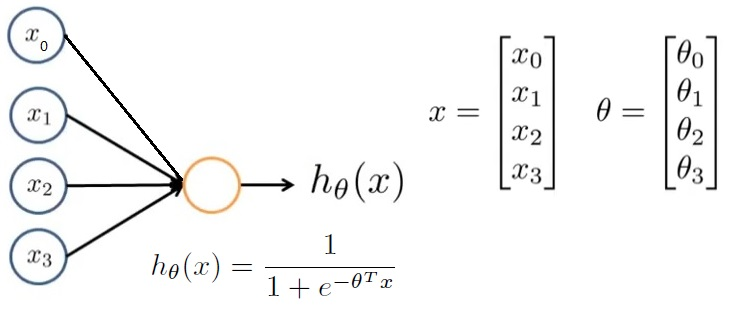
\includegraphics[width=5cm]{Figure2.jpg}\\
  \caption{Logistic Neuron Unit}\label{logistic_neuron_unit}
\end{figure}
\begin{figure}[ht]
  \centering
  % Requires \usepackage{graphicx}
  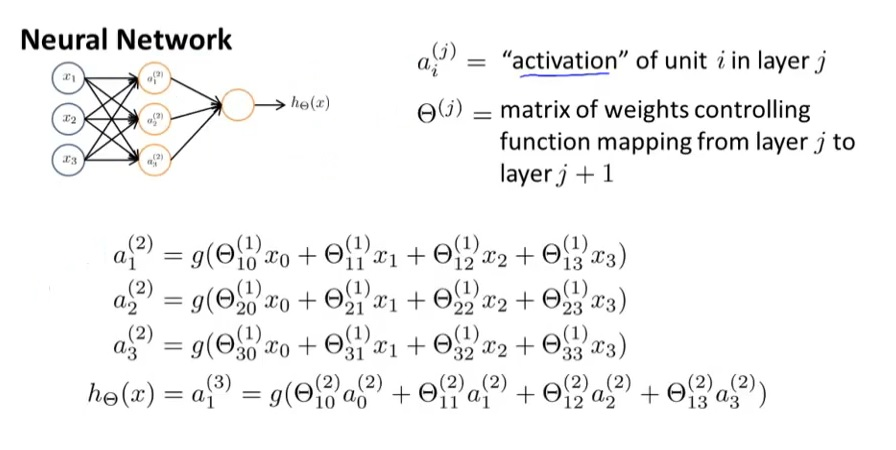
\includegraphics[width=9cm]{Figure3.jpg}\\
  \caption{Neural Networks}\label{neural_networks}
\end{figure}
\section{Motivation}
Let's see an classification problem shown in Fig. \ref{XOR_classification_problem}. Obviously, there does not exists a linear curve separating the two classes. However, a logic function of $x_{1}$ XOR $x_{2}$ classifies the two classes perfectly. Neural networks are good at these non-linear problems, and we can build a neural network to solve the XOR classification problem. Using the logistic neuron unit in Fig. \ref{logistic_neuron_unit}, we can first get three logic classifiers shown in Fig. \ref{logic_neurons}. To verify the correctness of these three logic classifiers, you may draw the truth table. Combining the three logic neurons, Fig. \ref{XOR_neural_networks} shows the final neural networks to solve the XOR classification problem with its truth table on the right.
\begin{figure}[ht]
  \centering
  % Requires \usepackage{graphicx}
  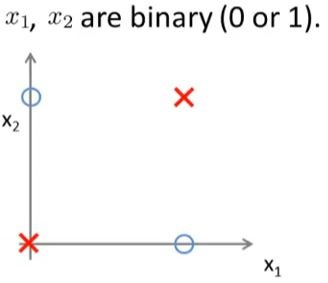
\includegraphics[width=3cm]{Figure4.jpg}\\
  \caption{Neuron Model}\label{XOR_classification_problem}
\end{figure}
\begin{figure}[ht]
  \centering
  % Requires \usepackage{graphicx}
  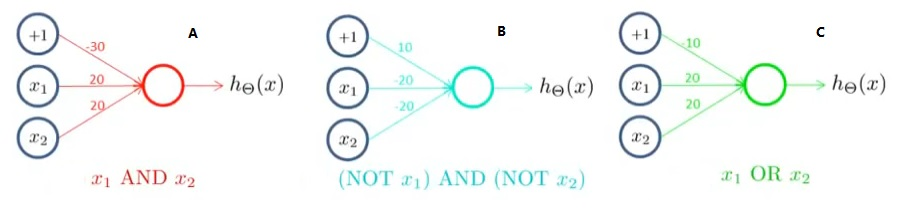
\includegraphics[width=10cm]{Figure5.jpg}\\
  \caption{Neuron Model}\label{logic_neurons}
\end{figure}
\begin{figure}[ht]
  \centering
  % Requires \usepackage{graphicx}
  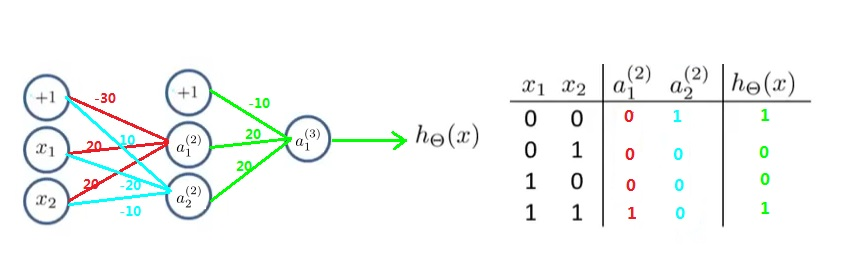
\includegraphics[width=10cm]{Figure6.jpg}\\
  \caption{Neuron Model}\label{XOR_neural_networks}
\end{figure}
\section{Cost Function}
Generally, neural networks outputs k hypothesis when solving a k classes classification problem. Using notations shown in Tab. \ref{neural_networks_cost_function_notation} and regularized logistic regression cost function, we can define the neural networks' cost function as shown in (\ref{}).
\begin{table}[hb]
\begin{center}
\caption{}\label{neural_networks_cost_function_notation}
\begin{tabular}{l|l}
\hline
Notation & Meaning\\
\hline
L   & total No. of layers\\
$s_{l}$ & No. of units in layer l\\
K   & No. of output units \\
$(h_{\theta}(x))_{i}$ & $i_{th}$ output hypothesis\\
\hline
\end{tabular}
\end{center}
\end{table}
\begin{equation}\label{neural_networks_cost_function}
J(\theta) = -\frac{1}{m}\biggl[\sum_{i=1}^{m}\sum_{k=1}^{K} y_{k}^{(i)}log(h_{\theta}(x^{(i)}))_{k} + (1 - y_{k}^{(i)})log(1 - (h_{\theta}(x^{(i)}))_{k})\biggr] + \frac{\lambda}{2m}\sum_{l=1}^{L-1}\sum_{i=1}^{s_{l}}\sum_{j=1}^{s_{l+1}}(\theta_{ji}^{(l)})^{2}
\end{equation}
The index of i starts from 1 instead of 0 is because the bias is always ignored to regularize. When running gradient descent algorithm, we need compute the partial derivative terms of $\frac{\partial}{\partial \theta_{ij}{(l)}}$ for all i, j, and l.
\end{document}
